\documentclass[12pt,letterpaper]{article}
\usepackage[margin=0.6in,headheight=15pt,headsep=16pt,footskip=22pt]{geometry}
\usepackage[T1]{fontenc}
\usepackage{helvet}
\renewcommand{\familydefault}{\sfdefault}
\usepackage{tikz}
\usetikzlibrary{arrows.meta}
\usepackage{fancyhdr}
\usepackage{parskip}
\pagestyle{fancy}
\fancyhf{}
\renewcommand{\headrulewidth}{0.25pt}
\renewcommand{\footrulewidth}{0pt}
\newcommand{\level}{Grades 2--5}
\fancyhead[L]{\fontsize{10.5}{12}\selectfont Week 79 / Numbered-ball detectives / \level}
\fancyfoot[L]{\fontsize{9}{11}\selectfont Bellingham Math Circle / Week 79 / 79-ST-v1}
\fancyfoot[R]{\fontsize{9}{11}\selectfont \thepage}
\setlength{\parindent}{0pt}
\setlength{\parskip}{9pt}
\pdfinfoomitdate=1
\pdftrailerid{}
\pdfsuppressptexinfo=15
\newcommand{\problem}[2]{\par\textbf{Problem #1:} #2\par}
\newcommand{\card}[3]{\draw[rounded corners=1pt,fill=white,line width=0.7pt] (#1-0.38,#2-0.38) rectangle (#1+0.38,#2+0.38);\node[font=\large] at (#1,#2){#3};}
\begin{document}
\fontsize{14}{18}\selectfont

Both bowls start empty. Each day, put the next two numbered cards in A, then move A's smallest card to B. Cards in B stay there.

\begin{center}
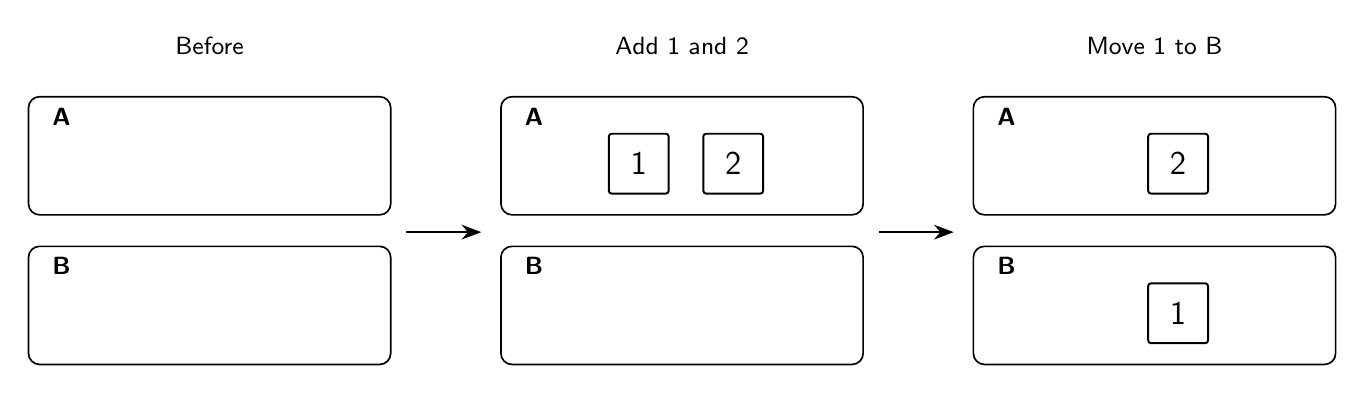
\begin{tikzpicture}[x=1cm,y=1cm]
  \foreach \x/\t in {3/Before,9/{Add 1 and 2},15/{Move 1 to B}} {
    \node[font=\small] at (\x,3.4){\t};
    \draw[line width=0.6pt,rounded corners=4pt] (\x-2.3,1.25) rectangle (\x+2.3,2.75);
    \draw[line width=0.6pt,rounded corners=4pt] (\x-2.3,-0.65) rectangle (\x+2.3,0.85);
    \node[font=\bfseries\small,anchor=west] at (\x-2.12,2.5){A};
    \node[font=\bfseries\small,anchor=west] at (\x-2.12,0.6){B};
  }
  \draw[-{Stealth[length=2.5mm]},line width=0.7pt] (5.5,1.03)--(6.45,1.03);
  \draw[-{Stealth[length=2.5mm]},line width=0.7pt] (11.5,1.03)--(12.45,1.03);
  \card{8.45}{1.9}{1}
  \card{9.65}{1.9}{2}
  \card{15.3}{1.9}{2}
  \card{15.3}{0}{1}
\end{tikzpicture}
\end{center}

\problem{1}{Run six days with cards 1--12. Can the bowls ever end a day with different numbers of cards? You may continue to twelve days with cards 1--24.}

\vfill
\begin{tikzpicture}[x=1cm,y=1cm]
  \draw[gray!55,line width=0.5pt] (0,0) rectangle (18.4,5.6);
\end{tikzpicture}
\vspace{0.2cm}

\newpage

\problem{2}{Restart. Find a rule for the day any numbered card moves to B. Test your rule on cards 3, 6, and 10, and predict the day for card 20 without running twenty days.}

\begin{center}
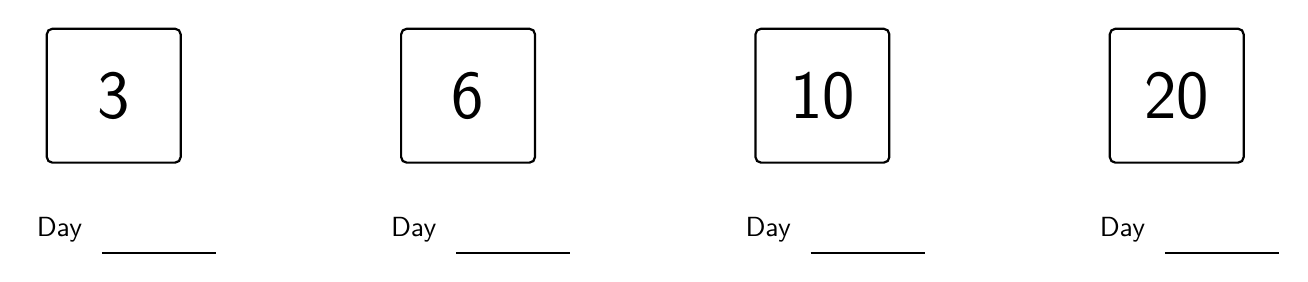
\begin{tikzpicture}[x=1cm,y=1cm]
  \foreach \x/\v in {2.3/3,6.8/6,11.3/10,15.8/20} {
    \draw[line width=0.8pt,rounded corners=2pt] (\x-0.85,1.1) rectangle (\x+0.85,2.8);
    \node[font=\fontsize{25}{28}\selectfont] at (\x,1.95){\v};
    \node[font=\normalsize,anchor=west] at (\x-1.1,0.25){Day};
    \draw[line width=0.5pt] (\x-0.15,-0.05)--(\x+1.3,-0.05);
  }
\end{tikzpicture}
\end{center}

\vspace{0.7cm}
\problem{3}{Start again. Each day, move the larger of today's two new cards to B, instead of A's smallest card. Could somebody tell which rule you used from the bowl counts alone? Find a way to show the difference using the cards.}

\vfill
\begin{tikzpicture}[x=1cm,y=1cm]
  \draw[gray!55,line width=0.5pt] (0,0) rectangle (18.4,5.6);
\end{tikzpicture}
\vspace{0.2cm}

\newpage
\renewcommand{\level}{Grades 4--5}

\problem{4}{Imagine the numbered cards continuing forever, with two new cards each day. Call a label settled in a bowl if, after some day, it stays in that bowl forever. For each rule, decide where all the labels settle. Can that arrangement happen on a finite day?}

\vspace{0.7cm}
\begin{center}
\begin{tikzpicture}[x=1cm,y=1cm]
  \node[font=\large] at (9.1,14.35){Move A's smallest card};
  \draw[line width=0.6pt] (0,7.4) rectangle (8.9,13.7);
  \draw[line width=0.6pt] (9.5,7.4) rectangle (18.4,13.7);
  \node[font=\Large,anchor=north west] at (0.25,13.45){A};
  \node[font=\Large,anchor=north west] at (9.75,13.45){B};
  \node[font=\large] at (9.1,6.65){Move the larger new card};
  \draw[line width=0.6pt] (0,0) rectangle (8.9,6);
  \draw[line width=0.6pt] (9.5,0) rectangle (18.4,6);
  \node[font=\Large,anchor=north west] at (0.25,5.75){A};
  \node[font=\Large,anchor=north west] at (9.75,5.75){B};
\end{tikzpicture}
\end{center}

\newpage
\renewcommand{\level}{Grades 2--5}

\begin{center}
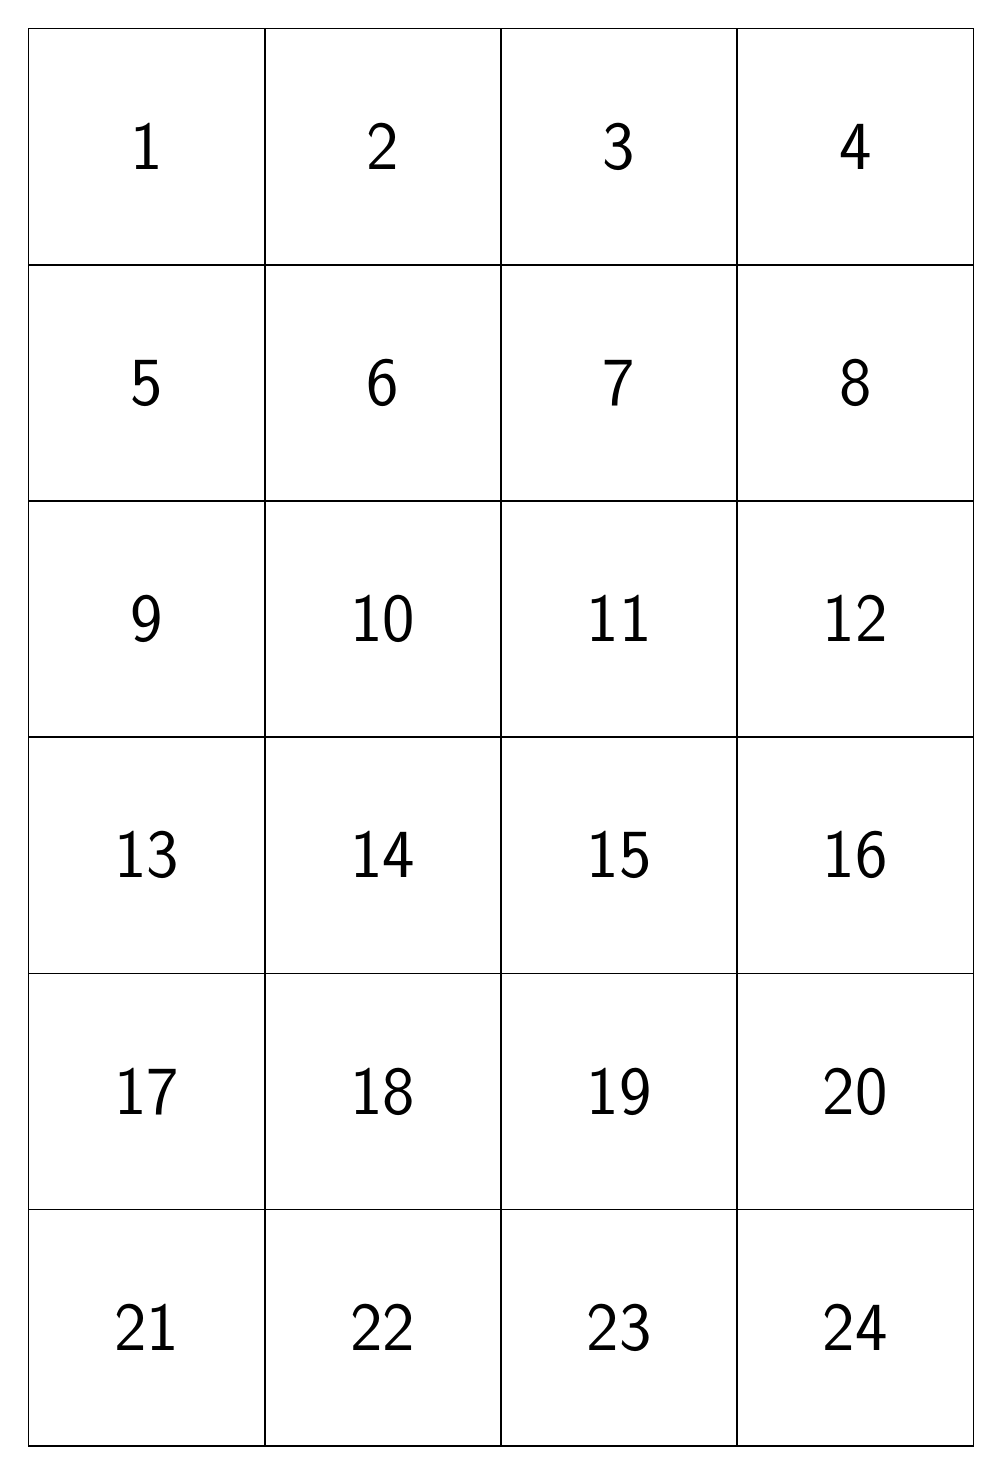
\begin{tikzpicture}[x=1cm,y=1cm]
  \foreach \r in {0,...,5} {
    \foreach \c in {0,...,3} {
      \pgfmathtruncatemacro{\v}{4*\r+\c+1}
      \draw[line width=0.6pt] (3*\c,-3*\r) rectangle (3*\c+3,-3*\r-3);
      \node[font=\fontsize{27}{30}\selectfont] at (3*\c+1.5,-3*\r-1.5){\v};
    }
  }
\end{tikzpicture}
\end{center}

\newpage

\begin{center}
\begin{tikzpicture}[x=1cm,y=1cm]
  \node[font=\fontsize{30}{32}\selectfont] at (9,21){A};
  \draw[line width=1pt,rounded corners=4pt] (0,10.6) rectangle (18,20.2);
  \node[font=\fontsize{30}{32}\selectfont] at (9,9.8){B};
  \draw[line width=1pt,rounded corners=4pt] (0,-0.6) rectangle (18,9);
\end{tikzpicture}
\end{center}

\end{document}
